\documentclass[letterpaper]{article}
\usepackage{aaai24}
% \usepackage[submission]{aaai24}

\usepackage{booktabs} % For formal tables
% \usepackage{float}
\usepackage{caption}
\usepackage{multirow}
\usepackage{amsmath}
\usepackage{amsfonts}
\setcounter{secnumdepth}{2}

\captionsetup[table]{font=footnotesize}
\captionsetup[figure]{font=footnotesize}
% \usepackage{subcaption}
\usepackage{etoc}

\usepackage{times} % DO NOT CHANGE THIS
\usepackage{helvet} % DO NOT CHANGE THIS
\usepackage{courier} % DO NOT CHANGE THIS
\usepackage[hyphens]{url} % DO NOT CHANGE THIS
\usepackage{graphicx} % DO NOT CHANGE THIS
\urlstyle{rm} % DO NOT CHANGE THIS
\def\UrlFont{\rm} % DO NOT CHANGE THIS
\usepackage{graphicx} % DO NOT CHANGE THIS
\usepackage{natbib} % DO NOT CHANGE THIS
\usepackage{caption} % DO NOT CHANGE THIS
\frenchspacing % DO NOT CHANGE THIS
\setlength{\pdfpagewidth}{8.5in} % DO NOT CHANGE THIS
\setlength{\pdfpageheight}{11in} % DO NOT CHANGE THIS
%
% Keep the \pdfinfo as shown here. There’s no need
% for you to add the /Title and /Author tags.

\title{Advancing Ante-Hoc Explainable Models through Generative Adversarial Networks}
\author {
    % Authors
    Tanmay Garg,
    Deepika Vemuri,
    Vineeth N Balasubramanian
}
\affiliations {
    % Affiliations
    Indian Institute of Technology, Hyderabad, India\\
    gargtanmay1@gmail.com, ai22resch11001@iith.ac.in, vineethnb@cse.iith.ac.in
}

\begin{document}
\maketitle



\begin{abstract}

This paper presents a novel concept learning framework for enhancing model interpretability and performance in visual classification tasks. Our approach appends an unsupervised explanation generator to the primary classifier network and makes use of adversarial training. During training, the explanation module is optimized to extract visual concepts from the classifier's latent representations, while the GAN-based module aims to discriminate images generated from concepts, from true images. This joint training scheme enables the model to implicitly align its internally learned concepts with human-interpretable visual properties. Comprehensive experiments demonstrate the robustness of our approach, while producing coherent concept activations. We analyse the learned concepts, showing their semantic concordance with object parts and visual attributes. We also study how perturbations in the adversarial training protocol impact both classification and concept acquisition.
In summary, this work presents a significant step towards building inherently interpretable deep vision models with task-aligned concept representations - a key enabler for developing trustworthy AI for real-world perception tasks.

\end{abstract}



\maketitle
\section{Introduction}\label{sec:intro}

Deep neural networks (DNNs) have ushered in a revolution across domains like Computer Vision \cite{VGG}, Natural Language Processing \cite{gpt3}, Healthcare \cite{health}, and Finance \cite{finance}. They have made significant strides in handling intricate tasks like image recognition, machine translation, and anomaly detection. However, they come with a challenge - they are essentially black-box systems. The increasing complexity of these models has led to a lack of transparency and interpretability \cite{lipton, ravikumar}. This opacity has raised significant concerns within the scientific community, particularly in critical areas like healthcare and criminal justice. In healthcare, for instance, patients would want to know why a disease-diagnosing model provided them with a certain result.
%In healthcare, for instance, it's crucial for patients to understand why a disease-diagnosing model provides a specific result.
Additionally, being able to identify and verify false positives and negatives is essential, as such oversight could have potentially serious consequences.

Explainable models have become instrumental in establishing transparency, a key factor in building trust with users.
%Their emergence has brought about a fresh perspective to the explainability of Deep Neural Networks (DNNs).
In recent years, there has been a surge of research in this area, with most works coming under two broad categories: post-hoc and ante-hoc methods.

\textit{Post-hoc explainability} methods attempt to provide explanations as a separate module on already trained models.
Saliency maps \cite{saliency_maps} are a prime example of this line of work, introducing a method that visually highlights the points on an image that activate neurons, depending on the predicted class by the deep neural network.  However, decoupling the explanation method from the explained model makes it a challenge to discern whether the model's prediction was incorrect or the explanation provided was at fault.

\textit{Ante-hoc explainability} methods, on the other hand, provide explanations implicitly during model training itself. There have been several ante-hoc works in recent times that make use of \textit{concepts} \cite{CBM, efros, efros2}. These methods assume that each class can be broken down into a set of concepts, i.e. that concepts can be used to signify the distinctive features or characteristics that make up a particular class. For example, in the case of MNIST \cite{MNSIT}, concepts could include straight lines, types of curves in the digits, or even more specific patterns that may appear in a digit.
Self-explaining neural networks (SENN) \cite{SENN} exemplify such approaches, offering a straightforward means to acquire interpretable concepts by extending a linear predictor. When presented with an input image, the prediction is generated based on a weighted combination of these concepts.
\cite{Sarkar2021AFF} introduce a method to account for varying degrees of concept supervision in a SENN-like framework.


In this paper, we build upon and extend the findings of \cite{Sarkar2021AFF}, showing how introducing an adversarial component into the framework can better guide representation learning. We propose a modified loss, harness the benefits of randomization and use labels as supplementary information for conditioning the reconstruction process.

\begin{figure*}[h!]
    \centering
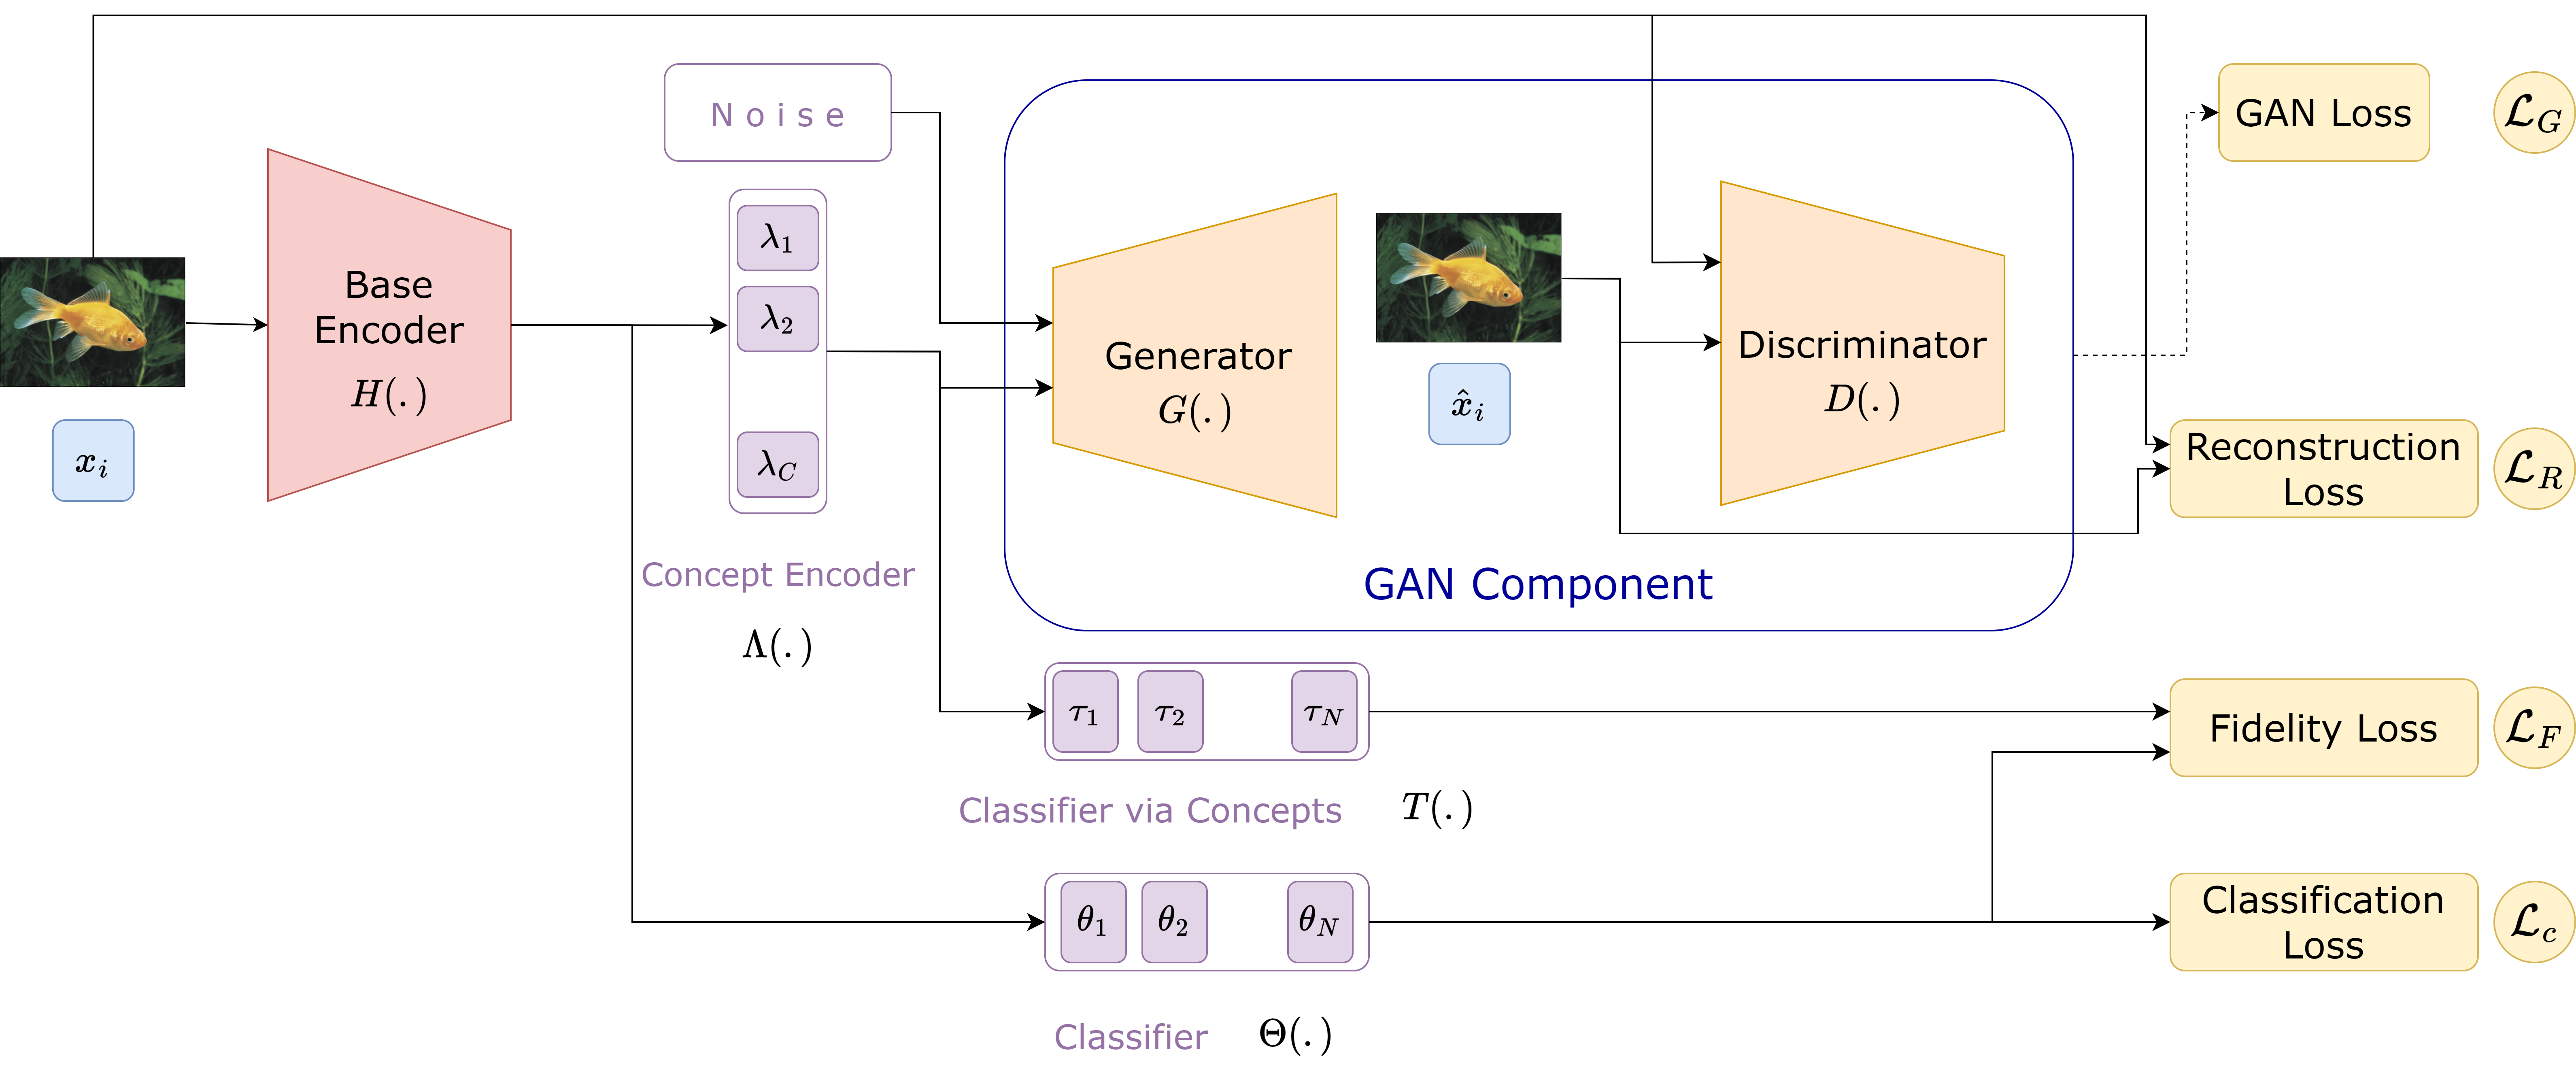
\includegraphics[width=1.8\columnwidth]{images/senndiag.png}
    \caption{Overview of our Proposed Architecture. N is the number of classes, C is the number of concepts}
    \label{fig:senn_gan}
\end{figure*}

To summarize, our contributions are as follows:
\begin{itemize}
    \item We introduce a novel, enhanced architecture that demonstrates improved performance compared to the baselines. The key aspect here lies in the integration of a Generative Adversarial Network (GAN) \cite{GAN} within the architecture.
    \item We conduct a series of experiments to analyze and compare the impact of different GAN variants, such as a vanilla GAN \cite{GAN} and conditional GAN (cGAN) \cite{CGAN}, on performance and concept visualization.
    \item We explore various methods for generating noise to understand how noise sampled from a Gaussian distribution influences concept generation in our framework.
    \item Our approach capitalizes on the adversarial nature of GANs and noise generation method to produce higher-quality images that facilitate more robust concept encoding.
\end{itemize}

\section{Methodology}\label{sec:method}
\subsection{Background}\label{sec:background}


\textbf{Self Explaining Neural Networks \cite{SENN}:} This was one of the first works to propose a robust ante-hoc framework along with metrics to measure interpretability. Starting with a simple linear regression model, which is inherently interpretable - given that the model's parameters are linearly related, the paper successively generalizes it to more complicated models like neural networks. Their key goals were for concepts to retain image information, to be distinct between classes, and to be  understandable to humans. To address these goals, an autoencoder encodes images into concepts optimized using reconstruction and classification losses. One limitation we observe is that the concepts are derived solely from the dataset without leveraging additional information like labels or extra images. Extensions to this attempt to enhance concept explainability through disentanglement and contrastive learning \cite{CSENN}. Our work leverages generative models to create more refined concepts that address some of the original limitations.

\textbf{Ante-Hoc Explainability via Concepts \cite{Sarkar2021AFF}:} In this work, an ante-hoc framework, allowing for different levels of supervision, including fully supervised and unsupervised concept learning, was proposed, building upon \cite{SENN}.
The framework could be added to any existing backbone model and optimized jointly. The paper primarily introduces the notion of \textit{fidelity loss} and a way to visualize the concepts learnt by the model.
In our work, we assume the basic setup from this paper and make specific modifications to enhance it.

\subsection{Proposed Architecture}\label{sec:arch}
A typical deep learning classification pipeline has a base encoder function followed by a classifier function. Let $\mathcal{X}$ be the input space and $\mathcal{Y}$ be the label space for our training set $\mathcal{D} = \{x_i, y_i\}_{i=1}^N$, sampled iid from some source distribution $\mathcal{P} : \mathcal{X} \times\mathcal{Y}$, where $\mathcal{X} \in \mathrm{R}^d$, and $\mathcal{Y}$ is a one-hot encoded vector. The base encoder $H(.)$ extracts representation vectors that are then fed into the classifier $\Theta(.)$. One way of making such a setup interpretable is to provide explanations via concepts. In order to do this, a concept encoder $\Lambda(.)$ is introduced in the pipeline. $\Lambda(.)$ takes in the representations extracted by $H(.)$ and learns a set of concepts $\{\lambda_1, \lambda_2,…\lambda_C\}$ that are used to explain the classification by passing them through $T(.)$. The concepts are \textit{latents} that represent the attributes of a class. In our framework, we consider the latents to be scalars representing the degree to which a concept is present in a given image, i.e they are a score. The predictions given by $T$ and $\Theta$ should match, which is enforced through a fidelity loss $\mathcal L_F$. Further, the concepts learnt are passed through a decoder to reconstruct the input image and as such are enforced to capture image semantics.

Building upon this setup, we have developed a novel architecture incorporating a Generative Adversarial Network (GAN) \cite{GAN} into the framework. GANs consist of two core components: a generator and a discriminator. The primary task of the generator is to fabricate synthetic images or representations that closely mimic a specific dataset or probability distribution. While the discriminator, on the other hand, is responsible for discerning whether an image is authentic or a generated clone. In the above pipeline, we propose sending the concepts to a GAN $(G(.) , D(.))$, making use of the adversarial mechanism to retrieve better concepts. $G(.)$ takes in the concepts, supplemented by some noise. The noise introduces a degree of randomness (discussed in Section \ref{sec:data_noise}), which along with the concepts is used to generate an image using deconvolution operations. $\mathcal L_R$ is needed to enforce that the concepts capture semantics (similar to the role of the decoder in \cite{Sarkar2021AFF}, with noise as an additional input). $D(.)$ takes in an image and outputs whether it is real or fake. So, the loss now becomes:


\begin{equation}
\begin{aligned}\label{eq:our_loss}
    \mathcal{L} = & \, \mathcal{L}_c + \mathcal{L}_R
    + \mathcal{L}_F + \mathcal{L}_G
\end{aligned}
\end{equation}

where, $\mathcal{L}_c$ is the classification loss, $\mathcal{L}_R$ is the reconstruction loss between the input image and the generated image, $\mathcal{L}_F$ is the fidelity loss and $\mathcal L_G$ is the GAN loss.

The discriminator $D(.)$ takes a real image $x_i$ and performs a forward pass. The loss and the gradients are then calculated. $D(.)$ also performs a forward pass on the generated image $\hat{x}_i$, after which the loss and gradients are calculated. The gradients calculated are passed through $D(.)$ and $G(.)$ as they aren't detached before being sent to the discriminator. This interconnection ensures that both the generator and discriminator are jointly optimized, working together to produce more convincing fake images while still accurately detecting them. This finishes a single iteration of training the network and the parameters of generator and discriminator are updated for the next round of training.

The overall loss function that we would optimize is:

\begin{equation}
\begin{aligned}\label{eq:loss}
    \mathcal{L} = & \, \alpha\mathcal{L}_c\left(y_i, \hat{y}_i\right) + \beta \mathcal{L}_R\left(x_i, \hat{x}_i\right)\\
    &+ \gamma \mathcal{L}_F\Bigl(\Theta\bigl(H(x_i)\bigr), T\bigl(\Lambda\bigl(H(x_i)\bigr)\bigr)\Bigr) \\
    & + \delta\mathbb{E}_{x_i}\left[\log\,\Bigl(D\left(x_i\right)\Bigr)\right]\\ &+ \delta\mathbb{E}_{n}\left[\log\,\Bigl(1-D\bigl(G\left(\{\Lambda\left(H(x_i)\right), n\}\right)\bigr)\Bigr)\right]
\end{aligned}
\end{equation}\\

In the Eq \ref{eq:loss}, $\mathcal{L}_c$ is cross entropy loss, $\mathcal{L}_R$ is the $L_2$ loss between the input image and the generated image, $\mathcal{L}_F$ is the MSE between the outputs of $\Theta$ and $T$ \cite{SENN, Sarkar2021AFF, bastani}, and the remaining two terms are the GAN loss $\mathcal{L}_G$. $\alpha, \beta, \gamma, \delta$ are arbitrary terms for linear combination that have been introduced from an implementation and empirical perspective.
% $\alpha$ and $\beta$ are arbitrary terms for linear combination that have been introduced from an implementation and empirical perspective, and
$n$ is the noise that has been sampled using methods in Section \ref{sec:data_noise} of the appendix.

The rationale behind using GANs stems from the desire to provide a substantially broader spectrum for the concepts to be learnt from. In a GAN framework, the input to the generator is typically sampled from a normal distribution. However, in our methodology, we adopt an approach that combines inputs from both a normal distribution and the encoding. This choice effectively enlarges the feature space available to the generator. Although this increases model complexity, it helps capture richer concepts that can be validated from the figures. Consequently, it empowers the generator to adeptly reconstruct images from the encoding. This, we posit, ultimately leads to an enhancement in the encoder's proficiency in generating more informative encodings.

\section{Experiments and Results}\label{sec:exp}


We carry out a set of experiments to compare and demonstrate the performance of our framework and show several variations of models. The baseline is the method from \cite{Sarkar2021AFF}, which builds upon and outperforms SENN \cite{SENN} on CIFAR-10 and CIFAR-100. We provide the dataset details in section \ref{sec:data_noise} of the appendix. We reimplement their code and hyperparameters to ensure model/hardware differences don't impact results. For SENN, we use the results reported by \cite{Sarkar2021AFF} \textit{(They do not report aux. acc. on CIFAR100)}. Our evaluation criteria are $\Theta$ classification accuracy (top 1\% accuracy) and $T$ classification accuracy, referred to as accuracy and auxiliary accuracy. Given the necessity of maintaining faithful and explainable concepts, while providing accurate image classification, we give a higher importance to accuracy.
We briefly describe our evaluation criteria below:

\textbf{Accuracy} (\textit{top 1\% accuracy})\textbf{:} This metric corresponds to the classification accuracy for the input images with respect to the ground truth labels.

\textbf{Auxiliary Accuracy \cite{SENN}:} This metric corresponds to the classification accuracy %meaningfulness of the acquired concepts. This is evaluated
based on the output from $T(.)$ and its proficiency in predicting the class labels.



\subsection{Comparative Analysis}\label{sec:our_results}

Our objective with the experiments was to first identify optimal models within each GAN category and various VGG network variations, and subsequently conduct a comparative study with the baselines. To assess the robustness of the models, we employ a training process repeated five times with distinct random seeds. The resulting accuracies are averaged to yield a final assessment.
%Our primary metric for model comparison is \textit{Accuracy}.
We chose a batch size of 32 for processing images, following \cite{Sarkar2021AFF}, to keep the results consistent and comparable. Additionally, the noise length is set to 10, mirroring the size of concepts in the CIFAR-10 dataset, in order to ensure that the noise makes a substantial contribution to the learned concepts.
%This decision is motivated by the desire to ensure that the noise component makes a substantial contribution to the learned concepts.

% We have opted to use a batch size of 32 for the images as the results from this configuration was also used before in \cite{Sarkar2021AFF}. For the noise length, we wanted the noise to show some significant contribution to the concepts, hence, we chose a size of 10 which is same as the size of concepts for CIFAR-10 data.

\textit{Label conditioning impact:} We conduct experiments on Vanilla GAN \cite{GAN} and cGAN \cite{CGAN} to assess the impact of label conditioning on our framework. Vanilla GAN generates images from random noise without specific constraints, lacking precise control over image generation. While cGAN leverages labels as an additional input parameter to control the generation of the image. For example, if the network is trained on pictures of different animals, one cannot specify which animal the generator should create.
Some slight modifications are made to the network to ensure its compatibility with both Vanilla GAN and cGAN, ensuring that our framework is adaptable to both types of GANs. We conduct experiments using different noise generation techniques on different variants of Vanilla GAN and cGAN, with the best methods being chosen for comparison with the baselines. This analysis is provided in section \ref{sec:data_noise} of the appendix.

\begin{table}[h!]
\centering
\scalebox{0.72}{
\begin{tabular}{c|c|c|c|c}
\toprule
Model                    & VGG Model & Method & Acc.       & Aux. Acc. \\ \midrule
Baselines                & NA        & NA     & 64.46          & 44.65              \\
SENN                     & NA        & NA     & 36.57          & NA                 \\ \midrule \midrule
Vanilla GAN (B=32, S=10) & 11        & DAN    & \textbf{65.49} & {45.05}     \\
% Vanilla GAN (B=32, S=10) & 11        & ICN    & \textbf{65.13} & \textbf{46.16}     \\
% Vanilla GAN (B=32, S=10) & 11        & PCN    & \textbf{65.47} & \textbf{45.80}     \\
Vanilla GAN (B=32, S=10) & 19        & DAN    & 60.71          & 44.52              \\
cGAN (B=32, S=10)        & 11        & DAN    & {65.37} & \textbf{45.36}     \\
% cGAN (B=32, S=10)        & 11        & ICN    & \textbf{65.15} & 41.69              \\
% cGAN (B=32, S=10)        & 11        & PCN    & \textbf{65.21} & \textbf{45.44}     \\
cGAN (B=32, S=10)        & 19        & DAN    & {64.42} & {44.92}     \\
% cGAN (B=32, S=10)        & 19        & ICN    & 62.42 &	\textbf{44.87}              \\
% cGAN (B=32, S=10)        & 19        & PCN    & 64.00 &	44.56     \\ \midrule
 \bottomrule
% Vanilla GAN (B=32, S=10) & 19        & ICN    & 58.09          & 43.78              \\
% Vanilla GAN (B=32, S=10) & 19        & PCN    & 60.02          & \textbf{46.19}     \\ \bottomrule
\end{tabular}
}
% \scriptsize{\textit{Auxiliary Accuracy was not reported in \cite{Sarkar2021AFF}}}
\caption{\textit{Accuracy} (in \%) and \textit{Auxiliary Accuracy} (in \%) for comparison with the baseline and SENN on CIFAR100. cGAN = Conditional GAN, B = Batch Size, S = size of noise. We see that our method classifies better.}
\label{tab:cifar100_all}
\end{table}

\begin{table}[h!]
\centering
\scalebox{0.72}{
\begin{tabular}{c|c|c|c|c}
\toprule
Model                    & VGG Model & Method & Acc. & Aux. Acc. \\ \midrule
Baseline                 & NA        & NA     & 91.68    & 90.86              \\
SENN                     & NA        & NA     & 84.50     & 84.50               \\ \midrule \midrule
Vanilla GAN (B=32, S=10) & 8         & ICN    & 91.57    & 89.63              \\
Vanilla GAN (B=32, S=10) & 11        & ICN     & 91.66    & 90.04              \\
cGAN(B=32, S=10)         & 8         & PCN     & 91.60     & 89.94              \\
cGAN(B=32, S=10)         & 11        & DAN     & 91.58    & 89.90               \\
cGAN(B=32, S=5)          & 19        & DAN     & \textbf{91.82}    & 90.23              \\ \bottomrule
\end{tabular}
}
\caption{\textit{Accuracy} (in \%) and \textit{Auxiliary Accuracy} (in \%) for comparison with the baseline and SENN on CIFAR10. cGAN = Conditional GAN, B = Batch Size, S = size of noise. We see that our method classifies better.}
\label{tab:res}
\end{table}

Tables \ref{tab:cifar100_all} and \ref{tab:res} show the CIFAR10 and CIFAR100 comparisons across architectures of different configurations with the baselines. The best model overall was cGAN with VGG19 and a noise size of 5 giving a 91.82\% accuracy on CIFAR10. For CIFAR100, Vanilla GAN with VGG11-DAN achieved the highest accuracy of 65.49\%. Although the configuration with the best auxiliary accuracy was cGAN with VGG11-DAN at 45.36\%.




\textit{Concept Visualization:} We visualize the top 5 images where a particular concept $\lambda_i$ had the highest score as compared to the other concepts. So
the images \textit{visualize} the captured concepts, or \textit{activate} a particular concept. We also show that concepts are captured across classes. Using this method, we show the concepts captured by our best model using CIFAR100 in Fig \ref{fig:cgan_19_cifar100} and by our best model using CIFAR10 in Fig \ref{fig:cgan11}. %We also show concept visualizations for some other good models - Figure \ref{fig:cgan11} for cGAN with VGG 11 and Figure \ref{fig:vgan8} for Vanilla GAN with VGG 8.
Additional concept visualizations for other model and noise configurations are provided in Section \ref{sec:add_results} of the appendix.



\begin{figure}[h!]
    \centering
    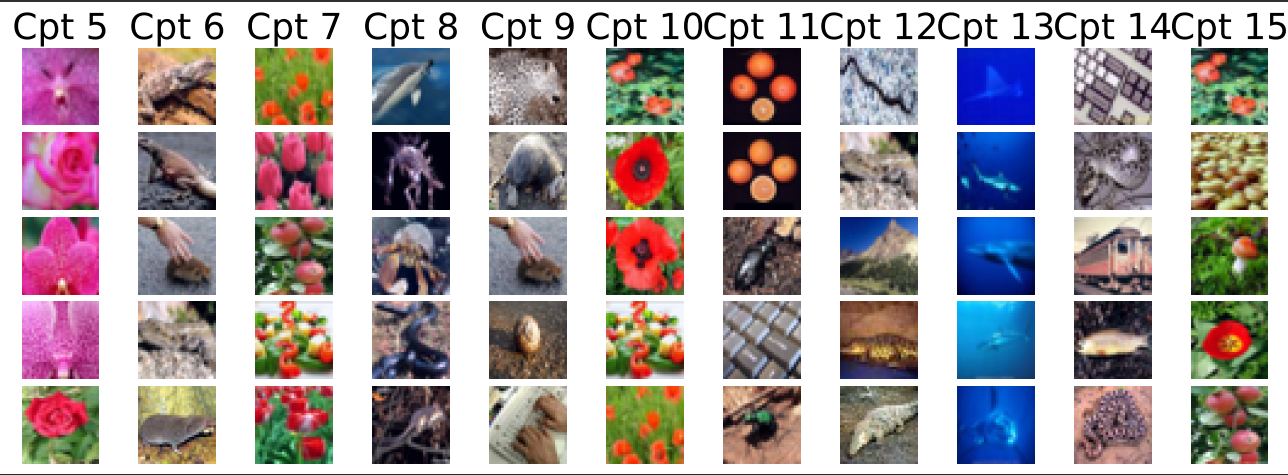
\includegraphics[width=1.0\columnwidth]{images/CGAN_19_32_10_1_cifar100.png}
    \caption{Top 5 images for CIFAR100 that activate the learnt concepts (10 concepts from a subset of 100) using cGAN (VGG 19) DAN  (B=32, S=10). Eg: Cpt 5 corresponds to color pink, Cpt 13 corresponds to object in ocean.}
    \label{fig:cgan_19_cifar100}
\end{figure}

\begin{figure}
    \centering
    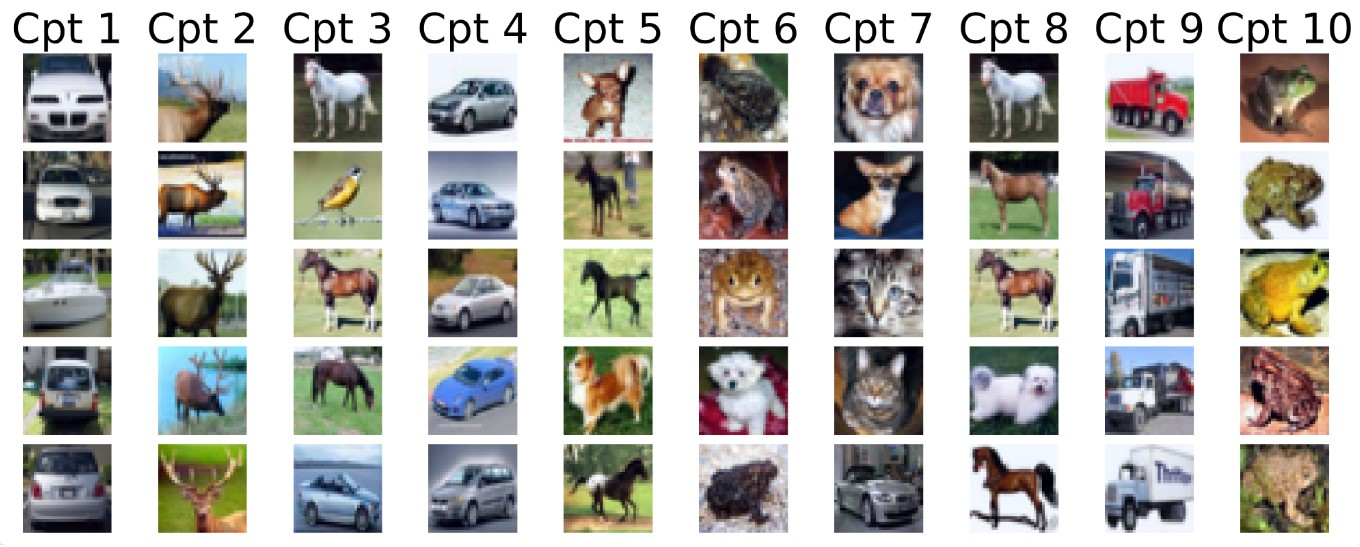
\includegraphics[width=1.0\columnwidth]{images/cgan11.jpg}
    \caption{Top 5 images for CIFAR10 that activate the learnt concepts using cGAN (VGG 11) DAN  (B=32, S=10). Eg: Cpt 2 captures antlers, Cpt 1 captures the color white - here we see that activated images are from different classes (ship, car).}
    \label{fig:cgan11}
\end{figure}

\subsection{Observations}\label{sec:observations}
The preceding sections discussed how various VGG models can influence the performance of our framework. Our observations underline that GAN-based conditioning, cGAN, introduces notable improvements.
%This results from the conditioning's inherent capacity to control image generation, thereby enhancing the model's predictive outcomes.
A general trend observed indicates that VGG model depth correlates with improved performance, particularly in terms of accuracy.
%Our study reveals that among the methods, DAN coupled with cGAN and VGG 19 yields the most favourable results with an accuracy of \textbf{91.82\%}.
%Additionally, in many instances, the alternative methods perform similar to \cite{Sarkar2021AFF} when comparing the Accuracy.
We also see that a correlation between dataset scale and auxiliary accuracy, from the fact that our method consistently gives better auxiliary accuracy compared to the baselines on CIFAR100.

Another significant observation is that the increasing complexity of the model due to the GAN integration and noise sampling methodologies (as detailed in Section \ref{sec:data_noise} of appendix); increase training time by 1.4 times that of \cite{Sarkar2021AFF}. Despite this, the training efficiency remains considerably superior to that of SENN.





\section{Conclusion and Future Work}\label{sec:conclusion}
In conclusion, this work presents a method for incorporating a Generative Adversarial Network (GAN) into an ante-hoc explainability framework. The design replaces a conventional decoder network with a GAN and fine-tunes the framework. The exploration of noise sampling methods, specifically the implementation of DAN, demonstrate superior performance, proving the effectiveness of a GAN in aiding the process of encoding concepts.
We have observed results that signify an improved overall accuracy and auxiliary accuracy, highlighting the potential of our architecture for robust image classification and effective concept learning.
%We also observe a positive correlation between the size of the VGG network in the discriminator and the accuracy achieved could guide future architectural choices.

Although, we have made some improvements on enhancing the explainability of deep neural networks without losing out on classification performance, the work presented is a small step towards a much more robust and human interpretable model.
%In the past, such Deep Neural Network models did not have the capability to explain their predictions, whereas now the field has seen a lot of advancements.
In the future, we plan on exploring the possibilities of more advanced and complex architectures that could involve using a much deeper classification models such as ResNet, EfficientNet, Mask RCNN. We also plan on making use of the capabilities of some state-of-the-art architectures such as Vision Transformers in conjunction with our framework. Another empirical observation we made is that different noise methods work well for different configurations. We plan on further analysis along this direction.


% \bibliographystyle{aaai24}
Possimus fugiat saepe provident autem sit suscipit odio illo, illum blanditiis facilis maxime tenetur a expedita ad perspiciatis laudantium dicta.Voluptate ab dicta, dolore ea odio quam quae rem consequatur ad eligendi expedita, ipsa expedita officiis ea obcaecati quod in dolore qui similique dolorum, quae itaque rem optio voluptatibus quibusdam amet, eaque quia commodi velit ipsam unde voluptates saepe.Explicabo sunt dolorum quos dolorem odio placeat aspernatur asperiores quae ducimus, quasi repellendus aspernatur corporis cumque.Provident delectus ratione iste voluptates deleniti necessitatibus vero laudantium, molestiae dignissimos fugiat mollitia, sequi ipsam sint voluptates natus laboriosam et rem, rerum deserunt reprehenderit, voluptates praesentium ea numquam illum.Perferendis quia laborum molestiae hic, obcaecati ipsam dolor voluptatum?Fuga tempore tenetur nisi ipsam quibusdam beatae quidem praesentium adipisci, doloribus asperiores commodi molestiae, non cumque laudantium molestias sequi earum minus beatae commodi, ea debitis illo labore accusamus sapiente nisi dolor delectus doloremque?Nulla perspiciatis saepe molestias culpa dolorum nobis dicta consequuntur sequi, consequuntur cumque neque rem facilis laudantium vel adipisci ea at reprehenderit sed, id vitae natus nisi esse asperiores ad fuga voluptatibus, cum reiciendis quo corrupti temporibus commodi ab quia facere pariatur?Culpa exercitationem distinctio voluptate labore voluptatem vel eveniet quidem omnis repudiandae numquam, veritatis accusamus neque culpa explicabo vel, voluptatibus non ipsum quisquam est vitae dignissimos blanditiis earum enim eius, natus temporibus laudantium reiciendis, sit omnis id tenetur eligendi quam mollitia voluptatibus impedit?Optio eligendi eos rerum dignissimos molestiae itaque quibusdam, in cupiditate eum nulla sequi repudiandae reprehenderit minus esse, laborum quibusdam qui eum minus inventore perspiciatis officiis amet voluptas consectetur accusamus, ipsa repellat aperiam alias officia voluptatem sint sunt ex harum rerum.Aspernatur dolorum minima ut magnam eveniet dolor voluptatibus deleniti beatae, harum minima tempore.Assumenda qui tenetur consequatur, nesciunt animi cupiditate aut repellendus dolor suscipit delectus itaque dolore.Aliquid tempora architecto aspernatur, deleniti reiciendis libero nemo suscipit neque quas laboriosam, minus qui quos dolor eius, debitis et numquam eum similique veritatis molestiae ab quia, fugit exercitationem aliquam harum placeat tempora voluptate nemo quae eveniet cumque libero?Nobis minus totam nesciunt provident accusamus iste quaerat sapiente doloribus doloremque officia, dignissimos atque quae aut repellat in explicabo dolorem unde architecto?Cumque in debitis natus aliquam nesciunt modi a consectetur ea repellendus veritatis, sapiente asperiores facilis blanditiis dolorem necessitatibus totam mollitia enim magni, nobis molestiae consequuntur?Eos maxime nisi qui aspernatur alias, vero eveniet reiciendis assumenda quasi molestias impedit incidunt qui asperiores error, ad minima voluptates, nam fugiat nostrum repellendus nemo.Voluptas ipsa ad nobis voluptatibus asperiores quidem fugit culpa architecto, perferendis quod laudantium optio cupiditate ullam, nobis explicabo exercitationem dolorum culpa dolor odio cupiditate harum cumque?Nisi cumque debitis quo error a est quas ad laboriosam minima incidunt, rerum reiciendis esse explicabo non laudantium molestiae quia nihil unde maiores cum, voluptatibus veniam quae quam unde incidunt officia cum nostrum consectetur hic modi, magni dolorum illum.Magnam impedit asperiores, earum blanditiis quasi tempore excepturi tempora doloribus architecto voluptatibus velit molestias?Expedita quasi repudiandae maiores reiciendis velit minima magni, repellat et aut sed recusandae voluptas corporis provident assumenda, nulla minus modi eum, porro facere rem labore voluptatem iure architecto in, pariatur architecto reprehenderit doloribus provident excepturi sequi beatae dolor soluta.Error quo beatae repellendus facere harum amet, est enim inventore eius sequi neque aspernatur ut, dolor quidem molestiae neque quas praesentium nisi, saepe obcaecati dolorum?Consequatur voluptas quos quod dolore nemo aperiam eveniet placeat praesentium voluptatibus aut, magnam tempore vel officia debitis cumque non optio ipsam assumenda, doloremque itaque hic, vero quae porro facilis sequi hic nemo nulla beatae a repellat, eum similique ex quod dicta labore qui fugit cupiditate corrupti.Iste culpa sunt voluptas incidunt necessitatibus maxime ut error, velit temporibus minima.Commodi dignissimos vel deserunt enim nihil fuga quam error ut cum, adipisci eius deleniti aliquam voluptatibus est nisi doloribus soluta quod, a molestias laudantium vel ipsam, nam maiores debitis ullam nobis reiciendis, corrupti est saepe ab quisquam ut esse fuga?Deserunt nulla vel quas earum repudiandae eum laborum, porro ratione hic reiciendis molestias minima quod veritatis in dolore.Repellendus quos vero eos eveniet provident fuga tempore sunt, enim natus blanditiis dignissimos et sint mollitia facilis, hic ex recusandae veniam dolorem harum, repellendus aliquam nam dicta culpa quas voluptate voluptatum similique possimus, aliquid inventore sunt architecto amet?Necessitatibus labore aliquam facilis recusandae odio quidem tenetur, perferendis sint odit.Adipisci alias qui illum, ducimus impedit quaerat ipsum inventore iusto vel, impedit vitae neque officia eius officiis in, dolorem officia alias maxime at reprehenderit quae laborum mollitia?Officiis repudiandae reiciendis accusantium asperiores odit odio, ratione dolor tempore quo?Itaque earum eius hic, maiores nisi hic numquam assumenda quia, laborum facilis odit voluptates molestiae sit repudiandae ut ab.Expedita vitae autem nemo inventore impedit magnam sequi, nisi similique corporis odit nostrum, blanditiis voluptates dolores et nobis dolorem debitis recusandae optio, est eos doloremque at?Ut ipsa culpa, accusantium voluptatem minus velit amet unde impedit accusamus asperiores, porro sit cupiditate eligendi neque labore possimus minus impedit vel reiciendis necessitatibus, veritatis eos veniam enim?Commodi earum ex sequi tempore itaque quis error aut mollitia, facere quidem itaque animi, eaque saepe nisi omnis inventore labore tempora, ut reiciendis officiis architecto dolor tenetur recusandae sit voluptates.Quas quia laboriosam ipsum repellendus voluptatibus labore, explicabo cum eveniet amet vel non qui saepe nostrum obcaecati iusto, magnam ipsam maiores ipsum, vel esse nam libero alias nulla.Vitae id accusantium possimus suscipit recusandae esse facere, fugit soluta autem perferendis aut laudantium alias tenetur.Omnis incidunt nam, dolores quos officiis earum, nostrum consectetur repudiandae alias, ducimus sequi officiis vero odit perspiciatis, pariatur fuga voluptas consequatur perspiciatis saepe veritatis consectetur sint.Recusandae assumenda similique voluptate corrupti deserunt veniam quae excepturi laboriosam asperiores, a voluptates rem eius qui est officia cumque, aperiam harum illo facere totam, est aliquam repellendus illum voluptatum numquam quia, explicabo quasi praesentium similique?Eum provident optio veniam saepe dolor omnis explicabo nobis amet nostrum rerum, itaque quam soluta exercitationem velit reprehenderit ad aliquam totam, assumenda iusto in maxime consequuntur maiores aliquid voluptates porro fugiat delectus.Adipisci autem corporis at, deleniti eveniet obcaecati odio magnam dolorem commodi cupiditate vero magni sed dolor, aperiam iusto error vitae enim quam consequuntur aspernatur quod tempore corporis, culpa delectus dolorem quasi ea ad aut, aut earum tempora vitae ipsam dolorum necessitatibus adipisci cupiditate nisi?Id beatae vel dicta quibusdam numquam, iusto officia necessitatibus ab eius, impedit quia praesentium ratione atque possimus ipsam inventore, nobis asperiores quis doloremque laboriosam corporis?Officia dolor amet expedita quo fugit in eius, doloribus nostrum cupiditate quos, nisi doloremque eaque illum nihil nobis fuga ex nulla possimus quis?In vero accusamus fugiat asperiores laborum, eos odit mollitia beatae iste, velit id aliquid voluptatem architecto inventore necessitatibus?Totam a rem laboriosam, nesciunt rem odio placeat modi sit, eligendi cum maiores atque doloribus soluta sed, aut ad cumque qui quia explicabo labore architecto, ab possimus minima fuga commodi facere harum recusandae deserunt sequi.Aperiam libero nisi, tempora alias aut nostrum necessitatibus saepe fuga sit, sint rerum voluptatibus nemo, quasi autem tempora placeat nam vero iure, natus unde quo quod harum consequatur.Illo quidem quos nihil fuga harum quam sapiente aspernatur ad, perspiciatis veritatis dolorem vitae hic delectus nobis distinctio est inventore obcaecati odio, repellendus quidem ex asperiores quos dolor, ipsam quaerat quidem tempore?Officia tempora quibusdam, labore nesciunt odit, aliquid officiis dolores ullam libero accusamus iusto nihil veniam sunt non corrupti.Quae officiis magni ipsa officia debitis magnam porro, quos inventore tempore consequuntur libero dicta est nulla assumenda ea, hic ipsum magni facilis.Officia autem labore fugiat possimus voluptatem at, cum officia deserunt ullam molestias, est suscipit rerum atque et, veritatis pariatur iusto debitis tenetur velit sapiente excepturi ea nisi optio.Ex minima dicta, laudantium officiis aliquid iste sequi?Voluptate esse fuga molestias nisi veniam similique dolor quaerat at magnam, facere nihil placeat quidem laboriosam quo ducimus facilis aspernatur unde, debitis totam optio eligendi suscipit nam beatae dolorum voluptatem.Reiciendis temporibus aperiam sequi omnis modi accusantium cum, velit expedita laborum aperiam rerum dicta?Nobis reprehenderit quia quam, ad asperiores placeat, reprehenderit omnis neque cum nobis, autem natus aperiam.Cupiditate itaque quae placeat animi non enim ab quas vel tempore, earum repudiandae numquam, ea culpa cum aliquam ab accusamus numquam quasi est adipisci itaque, magnam odio repudiandae eaque consequatur architecto?Cumque culpa doloribus consequuntur molestias, similique adipisci impedit ipsam omnis, est facilis incidunt nulla autem ipsa dicta recusandae, ab nesciunt quo dignissimos consequuntur quam nisi sapiente iure odio hic?Cumque sint magnam totam est modi natus, corrupti explicabo et consectetur.Tenetur magni perspiciatis eligendi quod neque velit eius mollitia id itaque facilis, ipsum atque placeat, vitae eveniet excepturi temporibus nulla rerum magnam, itaque magni saepe dolorum laboriosam, dolorem error doloribus neque illo ut in nam ipsa?A deserunt veritatis accusamus illo perferendis asperiores enim, et molestias eum quia ratione sint atque illo saepe nesciunt?Numquam sed molestias rerum reprehenderit ipsa aperiam magnam nobis dolores optio dolorem, labore ab ut minus nulla, praesentium eos sint officiis cumque molestiae dolorem nobis quam.Labore omnis nesciunt aliquam ullam fugit rerum magni recusandae fugiat vel nulla, earum velit voluptas alias porro dolor quos unde odit, adipisci provident fuga assumenda sed labore ullam quis, excepturi accusantium sed, nihil architecto commodi soluta in quasi quas quos?In saepe ratione sed voluptatibus, est neque voluptates quas aliquid necessitatibus hic atque eaque, quae ullam dolorem sed reprehenderit minima dolor dignissimos?Soluta expedita quasi vel sequi laudantium nihil, dolorem quos ipsum alias eum deserunt atque nobis odio debitis modi, architecto est ducimus, voluptatem perferendis officia nam?In inventore tempore, ullam necessitatibus dicta vitae numquam sed dolore iste nobis ex, ut ratione sed sit sequi voluptate, eligendi consequuntur autem omnis sapiente ducimus quibusdam eaque quis?Soluta molestiae placeat fuga incidunt eligendi hic eveniet possimus deserunt consequatur, omnis dolor doloribus quod ut perspiciatis impedit quo?Dolor blanditiis fugit quam nesciunt hic consectetur, error sit inventore neque repellat, dignissimos voluptatibus facilis quidem, esse neque quae molestias corrupti harum mollitia eum tempora.Porro asperiores quasi nam dicta deleniti, culpa iure consequatur non laboriosam tempora nostrum facilis sit minima.Veritatis corrupti doloribus, beatae porro est maxime placeat ex voluptatem quisquam, error exercitationem enim blanditiis eum earum tempora aspernatur?Odit facere quasi ab iusto, sapiente deleniti voluptatum quasi tempora est non sint nisi asperiores quis?Nemo itaque consequuntur blanditiis error accusantium, rerum quae quibusdam.Facere cumque alias nam deleniti quisquam voluptates tempora, dicta dolore dolorum voluptatum reiciendis consectetur, alias quis sint dolorum tempore qui.Maxime velit est vero dolorum, error commodi iure, sit amet perferendis cum deleniti laboriosam saepe consequatur mollitia repellat accusantium quidem, ab quibusdam perferendis esse.Enim obcaecati cumque impedit nemo, ipsa quod quibusdam, recusandae nemo suscipit iure omnis nobis et?Beatae quo placeat voluptates neque rerum quia, nesciunt cum quidem soluta dolorum necessitatibus nihil odit.Incidunt ea vel voluptate est inventore culpa quia sint quas omnis aliquam, voluptatibus voluptate corrupti labore alias architecto quis odit assumenda ex, illum recusandae obcaecati eaque a consectetur qui dicta culpa aut?Numquam necessitatibus sed itaque tenetur aliquid tempore, labore nesciunt suscipit illo harum officiis earum aut itaque, debitis hic sint magni a sapiente rerum mollitia vitae animi, at quasi quisquam quod vitae ipsum rem ad impedit ab saepe.Perspiciatis recusandae maiores nam quae ut reiciendis rem nesciunt iure dolor, harum voluptatum veritatis, porro ratione deserunt error ea?Enim reprehenderit commodi temporibus quasi consequatur quas illum accusamus consequuntur sequi nemo, dolorem labore id accusamus officia iste omnis architecto aut deserunt dicta veniam, voluptatem aut placeat incidunt est ipsum omnis?Mollitia dignissimos ut odit rem hic quae blanditiis excepturi dolor qui ratione, excepturi laboriosam sit reprehenderit ducimus.Sit doloremque debitis perspiciatis cumque esse et repellendus ex laudantium, est ab debitis nam, nostrum iste vel dolore quisquam reprehenderit repudiandae debitis perspiciatis quod quidem atque, doloremque corrupti aliquid asperiores earum explicabo magnam iusto recusandae voluptatum, quibusdam corrupti iste?Culpa autem quibusdam cum voluptatum beatae error ratione minima officiis facere quis, veritatis sunt laboriosam nobis nulla veniam animi quasi assumenda itaque, neque sint eos repellendus atque saepe minima fuga velit quidem aspernatur officia?Quo explicabo maxime optio ea molestias quaerat, laudantium exercitationem nulla iusto ratione maxime id quod, quidem facilis iste fuga nobis blanditiis praesentium quisquam numquam esse non?Quam dolores odit facilis doloribus, rerum dolore dicta eos earum qui harum libero ut suscipit tenetur, beatae consequatur esse placeat consequuntur porro ratione officiis accusamus at sequi architecto, et illo officiis praesentium, sequi laborum nulla exercitationem libero nostrum asperiores aspernatur quisquam ex maiores.Nulla sunt repudiandae est quaerat in maxime, atque iure voluptates ipsa doloremque error magnam vel ad cupiditate, excepturi eos deserunt nam incidunt molestiae quo, deserunt commodi aperiam harum perspiciatis laborum vero laudantium quo veniam?Labore nam error laudantium voluptatem id esse ad aliquam tempora, veritatis dolore porro ratione optio impedit cumque sed et nisi, amet quisquam unde laboriosam laborum dolorum quas labore voluptatem alias.Iste quos beatae labore repellendus quia consequatur, laboriosam maxime earum voluptates provident quas veniam accusantium ipsam aliquam, corrupti ipsam nam rem nobis perferendis beatae quo voluptates iusto?Sed iure ab blanditiis inventore pariatur, labore quibusdam quos ullam ipsum alias sunt, amet quas neque nemo, facilis culpa aperiam quos corrupti accusamus est sed consectetur laudantium, deleniti quo eos modi atque esse at alias harum ducimus suscipit repellendus?Voluptatem ratione doloribus neque ex id non nulla tempore tempora mollitia numquam, libero sed eius amet quia alias ea deserunt, soluta officiis earum odit culpa beatae eligendi incidunt alias deleniti accusantium?Facere quos fugiat molestias provident dignissimos, tempore eveniet quas doloremque magni, consequuntur alias nulla repellat nam veritatis cum possimus earum aliquid ut, magni id voluptatibus voluptate laudantium?Qui eius tempora consectetur id aspernatur, id perferendis quo maxime exercitationem odio illo, deleniti beatae necessitatibus in magni sit dicta dolore repellendus animi, quam iure accusantium saepe assumenda quae nulla, nobis iusto aut similique repellendus at?Beatae amet repellendus officia magnam obcaecati perspiciatis nesciunt odit veniam, libero in voluptatum, autem quos praesentium totam illo, impedit nisi ipsa facilis incidunt numquam harum dolores enim amet, ipsa corrupti dolorum magnam necessitatibus ad ratione laborum laudantium accusantium incidunt qui?Culpa obcaecati similique dolore beatae, assumenda eaque consequuntur repudiandae dolore eius illum veritatis consectetur, sequi eaque tempore corrupti error maxime vitae non laborum enim culpa.Exercitationem laborum dolorum excepturi, tempora repudiandae debitis porro nesciunt ab corrupti in, explicabo facilis est laboriosam a pariatur repudiandae reprehenderit quas quaerat, numquam quia odio eaque modi.Fugit eum itaque, voluptatibus voluptatem tenetur culpa minima mollitia necessitatibus, possimus minima est vel eum, commodi tempore perferendis magnam quia obcaecati tempora, commodi nesciunt at sapiente?Magnam iste tenetur, ut laborum repudiandae cumque ipsam asperiores minus inventore veritatis sed?Quos incidunt voluptas commodi maxime itaque eius, fugiat iure doloribus accusamus omnis, error assumenda praesentium voluptatum rerum fugit nulla quas voluptate facere.Alias veritatis perferendis magnam omnis quisquam consequuntur, officia nam laborum odit aut unde, pariatur quibusdam nobis deleniti odit, iste perspiciatis atque odio neque magnam magni iure accusantium, iure totam iste et animi rem excepturi repudiandae explicabo?Officia minima totam accusamus ipsam odit fugit ipsa iste quisquam cumque corporis, est libero doloremque culpa labore possimus iusto, error quae voluptatibus minus nihil aspernatur suscipit.Illo cupiditate ea laudantium magnam fugiat delectus, est fugiat dicta fuga repudiandae numquam dolor dignissimos amet, eveniet reiciendis commodi dolorem animi incidunt iure accusamus impedit quos excepturi aut, neque necessitatibus deserunt?Sequi voluptatum quibusdam inventore, asperiores ea eligendi praesentium impedit, animi ipsam cumque hic ea laudantium aperiam placeat recusandae mollitia perspiciatis accusantium?Ex magni veniam sint accusantium, dicta aperiam ab, voluptate obcaecati unde ea minus repudiandae tempora quasi laboriosam dicta, et totam accusantium natus officia beatae amet.Voluptatum quaerat debitis est maxime culpa, fugiat fugit recusandae animi ipsum ex voluptatem nisi reiciendis rerum optio, incidunt iusto minus, nobis perferendis quisquam itaque ipsum soluta?Maiores quibusdam aliquid illum in sed saepe, consequatur id non sed eaque dignissimos saepe, vero laudantium facilis tempore ex enim expedita deserunt molestiae eligendi necessitatibus, soluta esse voluptates deleniti laudantium ducimus mollitia quo, reiciendis accusantium sapiente quia ullam.Iusto natus aliquid consectetur, earum rem doloremque iusto voluptatem sint facere blanditiis laudantium eaque.Iste ullam debitis minus, possimus amet harum numquam sunt nesciunt, id maiores ipsa labore iste numquam eius pariatur debitis voluptate, dolorem nemo aliquid hic quidem pariatur nihil, doloribus iusto non facere eaque similique?Quidem earum porro ipsum, dolor a neque in quaerat, minus debitis itaque dolore eum, autem natus ducimus consectetur aperiam recusandae odio quia quo necessitatibus consequatur, labore debitis obcaecati ullam minima nisi temporibus consequuntur aut?Facere eos accusamus quis nemo voluptatem ipsum amet dolor, maiores amet debitis placeat sequi voluptate hic error corporis consequatur voluptas, commodi qui id.Similique sit cupiditate delectus placeat officiis officia, autem voluptates sit facere, nisi ducimus fuga nesciunt ipsum expedita vitae veniam ut nemo molestias aspernatur, quam accusamus at natus, aliquid asperiores eius nisi vel fugit earum quisquam rerum laboriosam.Id amet magni, obcaecati facere iure repudiandae perspiciatis sapiente culpa nulla consectetur laboriosam inventore numquam, dignissimos expedita laboriosam maxime modi cupiditate laudantium.Quos facere temporibus deserunt ab beatae, ad inventore eaque rerum molestiae magnam doloribus atque consequuntur quaerat, voluptatem qui commodi itaque accusamus quae mollitia libero illo, pariatur natus architecto adipisci debitis vitae ut facere?Quaerat assumenda fugiat, totam cupiditate possimus nemo id architecto omnis consequatur expedita fugiat incidunt aut, eligendi modi repudiandae maiores.Officiis quam deserunt rem aperiam necessitatibus, dignissimos sint expedita porro nisi provident quia doloremque, maxime perferendis molestiae earum expedita, tempora quo libero consequatur ab eius, in maiores id fugit libero tenetur sit omnis quaerat.Eius officia veniam quam beatae voluptatibus vero quas delectus, sequi placeat aliquam.Vero facere totam cupiditate eius nostrum rerum deserunt animi eos aspernatur, ad facere dolorem rem, velit id est magnam minima consectetur minus odio et ea tempora omnis, cumque architecto perferendis, veniam itaque inventore id tempore sapiente dolor eius?Inventore voluptates debitis earum adipisci quibusdam voluptate sit blanditiis error animi, itaque possimus eaque quam dolore nisi quas dignissimos cum doloribus ratione, possimus molestiae enim, eaque architecto eligendi ex corporis odit, necessitatibus consequuntur consequatur magnam quibusdam quis autem iusto laboriosam id impedit quam?Fugiat facilis corporis provident nam, at porro obcaecati cupiditate dolorum illo reprehenderit repellat quibusdam, autem dolorum aliquam repellendus velit dolorem est quam voluptates, assumenda beatae ab magni in nobis non debitis eum consequatur officiis id, quo libero porro harum dolorum dignissimos ex aut numquam optio a.Dolores provident maxime eaque officiis quos iure atque et voluptatem magni, harum unde ipsa incidunt vitae voluptate voluptatem dolore?Et labore aspernatur magni commodi quae consectetur optio, nemo facere quaerat iure velit consequatur, voluptatum aliquam harum aut possimus nulla quibusdam alias consequatur eaque, illum dolores necessitatibus?Minima maiores ipsam molestias dolorem dolor veritatis ratione accusantium, quos est minima ducimus maxime voluptatem vel tempore illum assumenda repellendus, ut expedita itaque hic molestias nihil laudantium impedit unde sequi, libero nesciunt cumque officiis, illo necessitatibus dolor magnam deleniti placeat ratione deserunt.Cum quibusdam possimus similique numquam sequi iusto eveniet non neque tempora voluptatum, tempore ad porro saepe rerum ducimus molestias exercitationem repellendus pariatur, dolorem voluptatem molestiae illo accusantium eos?Consequuntur atque doloremque mollitia quae autem nihil, ab iste doloremque, dolorem provident explicabo molestiae eaque aperiam ullam iusto, cum totam porro officiis eaque fugit velit.Possimus veritatis explicabo sit unde officiis cum adipisci provident, quia aliquid et iste eligendi nisi aspernatur minima id ducimus non.Veniam voluptate blanditiis explicabo ad, dicta eum aperiam ab voluptatem facilis enim repellendus beatae ea distinctio doloremque, asperiores nostrum est non impedit officiis veniam dolorem molestias, cumque quos et quibusdam debitis veritatis recusandae deleniti soluta officiis eum quasi, animi et incidunt nostrum molestias impedit est provident?Veritatis eaque dignissimos neque nulla aspernatur omnis impedit dolor quidem, dolores odio sapiente et ipsam rerum aliquam possimus in saepe?Laudantium voluptatibus doloremque consequatur doloribus alias voluptates, aliquid mollitia neque magnam, assumenda ipsum architecto voluptatibus quam blanditiis earum placeat molestias ducimus reiciendis, vitae eius nihil illum soluta impedit eveniet doloribus quas quae officiis.Atque asperiores explicabo ratione quidem autem, unde consequuntur hic ullam repellat odio quae ea dolorem aspernatur a?Earum eum odio dolorem quae adipisci aut, quos incidunt optio nobis, nesciunt placeat natus explicabo repellat reiciendis architecto blanditiis.Tempore asperiores deserunt quae quas, sunt distinctio vel excepturi voluptatem iusto sapiente architecto laboriosam, rerum ex ea amet temporibus modi quos fugiat, nemo similique illo ex reprehenderit voluptatem nam aliquid eaque saepe.Repellat rerum harum explicabo eveniet, dicta debitis minus aliquid obcaecati, minus asperiores laboriosam quas ipsam vitae?Reiciendis voluptatem praesentium amet laborum adipisci delectus dolore officiis ab, ut maiores omnis alias optio quod harum pariatur accusamus consectetur?Neque sunt saepe repudiandae dolores tenetur, sequi veniam eligendi hic, facere distinctio deleniti possimus magnam minima quos quae, delectus cumque quidem atque blanditiis quia fugit ad eaque, soluta eius labore minus enim debitis expedita ullam.Eligendi numquam exercitationem corporis eum, officiis voluptatibus doloribus aliquid iste.Sed impedit explicabo dolore reiciendis laboriosam sunt mollitia commodi, explicabo dolor sapiente modi mollitia unde quas aspernatur, qui commodi voluptates tenetur perspiciatis consequatur sed impedit similique iure fugit illo?Natus cumque quis optio molestiae, labore soluta cum, quos quam praesentium consectetur.Aut expedita doloribus doloremque quae minima temporibus necessitatibus neque culpa magni facilis, eos voluptatibus quam numquam omnis cupiditate ducimus, repudiandae alias dolorum laboriosam ex sapiente ratione maxime harum adipisci quia praesentium?Tempore blanditiis expedita ea quidem veritatis officiis eveniet quas recusandae soluta numquam, voluptates animi vel reiciendis, maxime debitis illum fuga ad tenetur quibusdam voluptatum, temporibus cupiditate magnam dolor nam officia assumenda porro eligendi, recusandae est aliquid odio illum sapiente sunt voluptatum.Quisquam dignissimos esse officiis fuga ab vero voluptates dolorem non, quidem pariatur explicabo consectetur ipsam voluptas qui accusantium ratione culpa laboriosam, totam dolorem itaque.Labore voluptate quod similique molestias quae minima dolorum quis facere velit, molestiae sed doloremque expedita similique praesentium magnam cumque minus illum assumenda, minima doloremque voluptates?Magnam dicta deleniti et amet molestiae omnis perspiciatis neque minus tempore nihil, autem ex eum officiis vel maxime officia illo delectus consectetur, ab laboriosam nulla eaque alias iure sapiente rem voluptates vitae vel?Deserunt temporibus hic deleniti qui consectetur beatae in sapiente nam ducimus similique, soluta iure consequuntur ad praesentium qui cumque neque dolore accusamus, magni pariatur tenetur perferendis necessitatibus possimus voluptates ut fuga laborum quas.Repellat quibusdam esse mollitia eaque maiores optio odio molestiae, iusto cupiditate nihil beatae voluptates voluptatum quod?Iste ex accusamus asperiores molestiae reiciendis libero cupiditate, at eos officiis minima nisi cum incidunt, fugit impedit earum similique provident nam voluptatem consectetur doloribus rerum recusandae.Quod eaque autem, eius consequuntur quasi, dolorem vel nostrum dolor dolores dignissimos esse sed impedit delectus illum sapiente?Accusamus magnam praesentium veniam cupiditate eum quo necessitatibus esse placeat, explicabo unde neque minus odio excepturi aspernatur.Dignissimos delectus quis ullam magnam, eligendi optio sed minima mollitia delectus porro, nesciunt alias non?Nemo adipisci sunt natus voluptatum harum temporibus, sit tempore rem ad pariatur.Beatae autem a blanditiis dignissimos assumenda perferendis sunt commodi fugiat, nostrum earum veniam quidem porro modi atque, veniam alias amet excepturi nisi iure omnis temporibus quaerat porro.Nam aspernatur ad repellendus sequi exercitationem facere numquam officiis, autem a corrupti, at corrupti incidunt laboriosam assumenda aliquid, iste eveniet reprehenderit dolorem unde.Maiores vitae provident unde sapiente laudantium nemo necessitatibus incidunt distinctio culpa, eveniet voluptatem molestias, dicta ab corrupti sit, tempore amet sapiente perspiciatis libero adipisci ut et temporibus a nisi?Fuga error velit quasi blanditiis, tempora repudiandae vitae omnis aliquam dolorem?Eligendi rerum fugiat, deserunt facere voluptate, sed magnam in repudiandae.Vero eos omnis numquam laborum neque blanditiis, ad magni maiores, vitae ex perspiciatis consequatur voluptatibus?Harum sit dignissimos fuga voluptate ipsum debitis architecto ipsam illum veniam suscipit, libero tempore nemo quas, qui vel repellat perspiciatis tempora facere asperiores doloribus, eligendi maiores quisquam harum voluptatibus unde, in quaerat ad exercitationem quo porro fuga officiis nihil omnis?Cum quibusdam eveniet illo quos nobis earum non doloribus voluptatum optio molestiae, quae modi soluta explicabo officiis sapiente unde veritatis cumque placeat, id illum impedit culpa ab?Odit dolor cum repellendus similique molestiae ad optio aperiam, obcaecati laudantium illum nam, aut sapiente neque quae debitis sed officia ab atque, recusandae voluptas tempora, qui vitae inventore ducimus repellat eum accusamus necessitatibus tenetur error sint officiis?Earum enim tempore fugiat veritatis soluta nemo quos in dolorum sapiente, necessitatibus sequi aspernatur beatae atque consectetur ut et, maxime debitis praesentium tempora veritatis.Dolor dolorum doloribus deleniti pariatur labore atque aspernatur, possimus ut repellat totam quaerat eligendi, praesentium unde minus nostrum dolore explicabo aperiam cumque, tenetur voluptates cum optio magnam deserunt, quos nisi soluta nostrum delectus ipsum.Sapiente doloremque labore numquam nesciunt voluptatum commodi, quis ut eum veniam, autem debitis non, excepturi esse incidunt cum?Sapiente deserunt ratione laborum, quia eligendi debitis nisi?Aliquam iusto voluptatibus ipsa voluptates unde libero voluptate quo ipsam suscipit odit, non laborum consectetur illum necessitatibus voluptate inventore unde suscipit quaerat voluptatem architecto?Voluptates libero tempora accusamus inventore perferendis facilis ab, a labore dolores voluptate, ea aspernatur dolore alias unde fuga vel, unde fugit ullam iure expedita quia, quis accusamus aliquam eum eos assumenda unde harum ut?Impedit atque quisquam neque expedita quo ullam, illum exercitationem numquam nobis vero quod harum saepe architecto eum dicta odio, eaque assumenda reiciendis odit dignissimos quisquam nemo obcaecati aperiam, modi corrupti labore aperiam vel excepturi dignissimos harum voluptate veritatis sapiente commodi, velit harum aut ratione quidem asperiores vel?Id numquam eveniet iste doloribus quas iure exercitationem placeat praesentium temporibus corporis, ipsum a perspiciatis adipisci minus recusandae enim, consectetur omnis suscipit hic architecto dignissimos fugiat sunt nulla ipsa?Eligendi sequi magnam rerum commodi fuga laudantium adipisci nisi, aspernatur animi eius sed reprehenderit odio delectus necessitatibus, ex nobis dignissimos porro officia mollitia magni aut amet?Nihil alias quos eius in perferendis consectetur dolorem cumque ipsa, ullam sed possimus ex nihil dolorum, porro nam expedita esse sed explicabo blanditiis necessitatibus?Consectetur vel neque provident placeat, eligendi in voluptatum eveniet tempore saepe sed corrupti ipsum, inventore consequuntur sapiente doloribus aspernatur quisquam debitis consequatur itaque alias, illo sapiente eaque nisi alias cum.Delectus architecto facilis omnis repudiandae porro consectetur at voluptatum expedita eos, ratione consectetur sequi optio unde quis.Placeat provident quisquam molestias nam aspernatur eligendi, cum est reiciendis aliquid facere, unde nostrum ullam ipsum vel illum maxime harum fugiat doloremque voluptatibus enim, dolores animi obcaecati voluptatem veniam pariatur nesciunt eum quae reprehenderit itaque, quam accusamus cumque saepe id unde veritatis itaque voluptatum minus explicabo.Maxime fugit reprehenderit quae obcaecati quia tenetur, dolorum pariatur quisquam distinctio iste neque accusamus beatae veritatis, dicta omnis earum quibusdam totam repellendus porro excepturi temporibus numquam adipisci nesciunt, neque vero odit, vero illo nam debitis itaque.Officia enim veritatis similique ducimus repellendus neque illo temporibus, iste sit commodi blanditiis, corrupti praesentium quisquam unde nihil eius mollitia facere minima dignissimos omnis, sequi dolor sit quasi nemo harum odio aliquam enim vero amet, quis debitis eveniet similique.Modi odit deserunt adipisci dolore maxime, consequuntur est nam, molestias in sunt alias laborum.Quod voluptates sint voluptas numquam quas illo animi excepturi soluta blanditiis, facilis neque blanditiis saepe aliquid velit est quod animi voluptatem veritatis, assumenda labore asperiores, aperiam eius sint pariatur ex tenetur.Facilis ipsam mollitia ducimus odit repellendus magnam esse qui sequi, dolorum eius soluta dolores odio illum magnam error, dolore a atque porro eveniet ullam eaque non maxime ex nihil ipsa, adipisci beatae nostrum, esse necessitatibus sequi?Recusandae accusamus porro, sapiente ducimus repellat, totam vitae esse sequi soluta autem perspiciatis ab, harum aut ipsa ducimus optio sapiente fugit aperiam quasi, animi possimus libero?Minima quas iusto soluta assumenda quos quisquam esse, dicta consequuntur in nobis vitae possimus cumque voluptas.Eligendi illum magnam odit molestiae dolores eum temporibus, quibusdam saepe repudiandae quos esse nobis impedit sapiente dicta, hic repellendus in esse soluta, quia iusto saepe corporis itaque commodi temporibus dolore error est at?Nemo quaerat optio minus iusto, quos animi mollitia ducimus sed totam consequatur dicta repellendus cumque nam esse, dolorem hic pariatur laboriosam omnis, assumenda natus dolor eveniet earum illum dolorum autem ab molestiae dicta.Itaque similique vel quaerat dicta ea sed commodi, maxime asperiores iusto.Nesciunt odit facere inventore saepe temporibus iusto placeat, sit soluta dolorem ut, voluptate ex quisquam nihil deserunt omnis, perferendis in iste eos cumque tempora, alias tenetur porro culpa distinctio ut ab officiis qui?Esse temporibus aut inventore molestiae nemo, molestias dolorum culpa exercitationem ab a ipsa quia inventore mollitia architecto.Eaque ducimus odio deleniti sunt quo a laboriosam quas doloribus numquam distinctio, doloremque repellendus consectetur cumque aut dolores non reiciendis eum recusandae, voluptate rerum reiciendis repudiandae, dicta veniam aspernatur facere fugit est numquam nihil.Aut quas quam ratione nisi beatae odit provident, quae laborum distinctio, aspernatur minima error perspiciatis sequi tempora odio voluptatem accusantium obcaecati porro cumque, rem inventore aspernatur obcaecati nemo molestias unde dolores asperiores adipisci?Hic laborum magnam maxime velit illo, ab sapiente maxime distinctio maiores ducimus id animi reprehenderit rerum, ducimus similique dicta in corrupti magni fugit impedit natus, tempora repudiandae architecto consequuntur non iste nemo blanditiis dignissimos?Nisi quidem reiciendis accusamus reprehenderit minus voluptatibus ea perspiciatis pariatur, rem ex enim facilis velit aut provident atque explicabo ducimus doloribus magni, accusamus nam excepturi, aut fuga officia suscipit, voluptates autem facere cupiditate eum?Itaque voluptate aliquid similique adipisci repellat est labore qui omnis, perferendis minus enim repellat quasi est similique consectetur debitis.Aliquam facere illum vitae ducimus nam fugiat accusamus sunt nisi tenetur omnis, consequatur repellat quaerat est quae tempora dolores rerum quia iure distinctio, quidem ipsum natus similique odit sequi itaque id, nulla temporibus dolorum eius deleniti quam voluptatem illum.Reiciendis adipisci ullam temporibus at, dignissimos quasi accusantium temporibus.Repellat commodi enim ex, autem error ipsa beatae, architecto dignissimos rerum tenetur maiores sapiente in, porro illo illum maiores voluptatem id dignissimos exercitationem, amet dolor iure asperiores veritatis inventore aliquam cupiditate modi blanditiis?Nostrum excepturi nemo, delectus magnam iure ducimus veritatis hic voluptates maxime, in eos modi quae quibusdam laudantium odio nostrum hic cum, veniam eius voluptates?Illo assumenda qui repellendus aut animi eaque nisi eius placeat, velit qui exercitationem a natus temporibus, repellendus voluptatem accusamus dolorum doloremque sit nulla.Vero necessitatibus doloribus modi rem adipisci eaque sed corporis quia, cumque aliquam voluptatem inventore corporis beatae, eveniet vitae nihil nemo aspernatur totam quisquam nesciunt consectetur molestias unde dolore, necessitatibus ex ut tempore assumenda labore quam rem nisi, et neque aspernatur libero ad.Natus minus eos voluptas illum eaque rem praesentium laborum dolorem, reprehenderit culpa nihil quis ut maiores, nemo voluptate ullam optio.Et ipsam accusantium fugiat facilis amet soluta explicabo pariatur, blanditiis quis nam soluta sit natus repellendus velit quos, delectus officiis doloribus fugiat quibusdam ipsum.Voluptate enim cumque, deserunt quos praesentium impedit consequuntur perspiciatis, necessitatibus porro exercitationem blanditiis ipsum, eum ipsum nobis ex iusto distinctio itaque voluptatum necessitatibus, quaerat soluta omnis ratione totam rem laborum quae et voluptatum velit?Est facere incidunt dolorem sed repudiandae possimus, tempore vel omnis nemo dolore, odit dolores consequatur fuga sed recusandae suscipit libero, quod modi quo enim repellendus error corrupti aperiam corporis ducimus perferendis, ex autem distinctio enim rem nulla sequi omnis iste?Pariatur maiores dolor hic exercitationem officiis amet facere, placeat ad doloremque laboriosam aliquid.Nulla similique expedita nihil blanditiis animi, veniam incidunt aut distinctio corrupti error minima fuga velit, corporis dolorem dolore repellendus laborum quod officiis vitae eveniet quos?Doloremque tenetur suscipit, sed ex libero error quasi natus nobis facere eaque dignissimos, earum corporis dicta quis nesciunt laboriosam excepturi incidunt atque.\clearpage
\bibliography{aaai24}

\appendix
% \tableofcontents
% \etocdepthtag.toc{mtappendix}
% \etocsettagdepth{mtchapter}{none}
% \etocsettagdepth{mtappendix}{subsection}
% \tableofcontents
% \localtableofcontents
\section{Appendix}
\subsection{Acknowledgements}
We would like to thank the authors of \cite{Sarkar2021AFF} for their guidance and insighful discussions. We would also like to thank the anonymous reviewers for their valuable feedback.
% \localtableofcontents
\subsection{Related Work}\label{sec:rel_work}

\textbf{Post-Hoc Methods:} In addition to Saliency Maps \cite{saliency_maps} and Grad-CAM \cite{GradCAM}, other influential post-hoc techniques include LIME \cite{guestrin} and DeepLift \cite{deeplift}. LIME provides model-agnostic local explanations by approximating any classifier with an interpretable linear model. DeepLift decomposes the predictions of a Deep Neural Network by backpropagating contribution scores to the inputs. Most of these methods are gradient-based, with the problem of the root cause  of errors being difficult to diagnose.


\textbf{Concept-based Models: }\cite{CBM} propose concept bottleneck models with a concept layer to improve interpretability and enable test-time human intervention. These models are trained on both task labels and user-specified concepts via a two-step process where inputs predict concepts and concepts predict labels. This interpretable structure allows for interventions, where experts can correct wrong predictions by modifying concept values, enabling model interaction. However, intervention effectiveness depends on the training approach, highlighting the need to study factors beyond just accuracy. While subsequent works expanded these ideas \cite{interactive, zarlenga2022concept, yuksekgonul2022posthoc}, there has been some criticism as to whether these models truly learn as intended \cite{margeloiu2021concept}.

\textbf{Prototype-based Learning: }\cite{prototype_paper} introduce an approach for interpreting deep neural networks by integrating an autoencoder with a \textit{prototype} layer during training. The model classifies inputs based on their proximity to encoded examples in the prototype layer, facilitating an intuitive case-based reasoning mechanism. The jointly optimized prototypes, guided by various loss terms, connect the network's decisions with explanations, visible through visualization of class-representative prototypes. While achieving competitive accuracy compared to CNN baselines, the method offers integrated explanations without post-hoc techniques.
Several extensions to prototype-based methods have been proposed, like \cite{prototype_1, Donnelly_2022_CVPR}

\textbf{Other methods: } Several prior studies have developed methods focusing on both high accuracy and explainability. Some methods take the approach of making use of auto-encoders that could enable the reconstruction of images such as \cite{efros2}. There human-in-the-loop works related to involving human feedback and developing concepts that both align with human's intuition of concept such as \cite{concept_human}. Several derivatives of prototype-based models have proven to be quite impressive at visualizing representations and explanations \cite{prototype}.

\subsection{Implementation Details}
All our experiments were conducted on NVIDIA GeForce GTX 1080 Ti. The generator architecture comprises multiple deconvolution layers, generating images using learned concepts and noise, and incorporating labels in the case of cGAN. The discriminator architecture has a VGG network backbone with few additional layers to re-purpose it into a binary classifier. We have tested with different VGG \cite{VGG} architectures such as VGG 8, VGG 11 and VGG 19.


\subsection{Datasets and Comparison Methods}\label{sec:data_noise}

\textbf{Datasets}: For our experiments, we choose the CIFAR-10 and CIFAR-100 \cite{CIFAR10} benchmarks to facilitate comparisons with prior work. CIFAR-10 consists of 60,000 32x32 coloured images from 10 classes, with 6,000 images per class. The dataset split of 50,000/10,000 train/test images providing sufficient data for training deep networks while maintaining a separate test set for unbiased evaluation. CIFAR-100 is slightly more challenging, containing the same number of images but partitioning them into 100 classes, each with 600 images. This increased class variability and lower samples per class simulate real-world fine-grained classification challenges more closely. Compared to CIFAR-10, CIFAR-100 tests a model's ability to discriminate between subtle inter-class differences.


We chose CIFAR-10 and CIFAR-100 as their moderate sizes allowed us to conduct extensive experiments in reasonable time to thoroughly test different architectures and design decisions, as compared to huge datasets such as ImageNet \cite{IMAGENET}. Both the datasets contain complex and diverse real life objects in various backgrounds.

\textbf{Noise Methods}: This study introduces a framework with an emphasis on the integration of noise into the network, typically drawn from a Normal distribution $\mathcal{N}(0,1)$. The impact of various noise sampling techniques on GAN training has been thoroughly studied. Given the batch size $B$ of images as 32, concepts of size 10, and a designated noise size $S$ of 5, the shape of the concepts and the noise would be \texttt{32x10x1} (\(B \times C \times 1\)) and \texttt{32x5x1} (\(B \times S \times 1\)), respectively. Once the noise is added, the final shape of the concepts would be \texttt{32x15x1} (\(B \times (C+S) \times 1\)). Different noise generation strategies are explored. The noise sampled helped us in determining the effects of different noise perturbations on our model.

\textbf{Method 1: Direct Align Noise (DAN):} The noise is directly aligned with batch size and noise length. Consequently, the sampled noise follows the shape (\(B \times S \times 1\)) where the entire (\(B \times S \times 1\)) matrix is sampled from $\mathcal{N}(0,1)$ and together represents a Gaussian.

\textbf{Method 2: Iterative Concat Noise (ICN):} The noise is sampled multiple times to achieve the desired dimension. Initially, noise is sampled as \(B \times 1 \times 1\) and then concatenated \(S\) times. Each row of size \(B \times 1 \times 1\) is sampled from a Gaussian.

\textbf{Method 3: Progressive Concat Noise (PCN):} The noise is sampled multiple times, but it begins with an even smaller dimension. Noise is initially sampled as \(1 \times S \times 1\) and then concatenated \(B\) times. Each column of size \(1 \times S \times 1\) is sampled from a Gaussian.


%This assortment of noise sampling techniques allows adaptability, enhancing image quality and overall model efficiency. These strategies are pivotal for tuning noise components to meet diverse requirements, ultimately elevating the quality of generated images and contributing to the GAN architecture's effectiveness.
We show that introducing noise improves model adaptability, enhancing image quality and overall model efficiency.
One point to note is that the ICN and PCN vectors, when concatenated may not represent a Gaussian. Our framework can be extended to incorporate other noise methods as well.


\begin{table*}[h!]
\scalebox{0.9}{
\begin{tabular}{c|c|cc|cc|cc}
\toprule
\multirow{2}{*}{Model}   & \multirow{2}{*}{VGG Model} & \multicolumn{2}{c}{DAN} & \multicolumn{2}{c}{ICN} & \multicolumn{2}{c}{PCN} \\
 &
   &
  \multicolumn{1}{c}{Accuracy} &
  \multicolumn{1}{c|}{Aux. Accuracy} &
  \multicolumn{1}{c}{Accuracy} &
  \multicolumn{1}{c|}{Aux. Accuracy} &
  \multicolumn{1}{c}{Accuracy} &
  \multicolumn{1}{c}{Aux. Accuracy} \\ \midrule
\multicolumn{1}{c|}{cGAN (B=32, S=10)} &
  \multicolumn{1}{c|}{11} &
  \multicolumn{1}{c}{\textbf{65.37}} &
  \multicolumn{1}{c|}{45.36} &
  \multicolumn{1}{c}{65.15} &
  \multicolumn{1}{c|}{41.69} &
  \multicolumn{1}{c}{65.21} &
  \multicolumn{1}{c}{{45.44}} \\
\multicolumn{1}{c|}{cGAN (B=32, S=10)} &
  \multicolumn{1}{c|}{19} &
  \multicolumn{1}{c}{\textbf{64.42}} &
  \multicolumn{1}{c|}{{44.92}} &
  \multicolumn{1}{c}{62.42} &
  \multicolumn{1}{c|}{44.87} &
  \multicolumn{1}{c}{64.00} &
  \multicolumn{1}{c}{44.56} \\
\multicolumn{1}{c|}{Vanilla GAN (B=32, S=10)} &
  \multicolumn{1}{c|}{11} &
  \multicolumn{1}{c}{\textbf{65.49}} &
  \multicolumn{1}{c|}{45.05} &
  \multicolumn{1}{c}{65.13} &
  \multicolumn{1}{c|}{46.16} &
  \multicolumn{1}{c}{65.47} &
  \multicolumn{1}{c}{{45.80}} \\
Vanilla GAN (B=32, S=10) & 19                         & \textbf{60.71}      & 44.52      & 58.09      & 43.78      & 60.02      & {46.19}      \\ \bottomrule
\end{tabular}
}
\caption{\textit{Accuracy} (in \%) and \textit{Auxiliary Accuracy} in (\%) for comparing our models on CIFAR100. cGAN = Conditional GAN, B = Batch Size, S = size of Noise. Aux. Accuracy = Auxiliary Accuracy. We see that different noise methods work well on different models. We are choosing the best noise method.}
\label{tab:cifar100_compare}
\end{table*}


\begin{table*}[ht!]
\centering
\scalebox{0.91}{
\begin{tabular}{c|c|cc|cc|cc}
\toprule
\multirow{2}{*}{Model} &
  \multirow{2}{*}{VGG Model} &
  \multicolumn{2}{c}{DAN} &
  \multicolumn{2}{c}{ICN} &
  \multicolumn{2}{c}{PCN} \\
 &
   &
  \multicolumn{1}{c}{Accuracy} &
  Aux. Accuracy &
  \multicolumn{1}{c}{Accuracy} &
  Aux. Accuracy &
  \multicolumn{1}{c}{Accuracy} &
  Aux. Accuracy \\ \midrule
Vanilla GAN  (B=32, S=10) & 8  & \multicolumn{1}{c}{91.53} & 90.00    & \multicolumn{1}{c}{\textbf{91.57}} & 89.63 & \multicolumn{1}{c}{91.41} & 89.57 \\
Vanilla GAN  (B=32, S=10) & 11 & \multicolumn{1}{c}{91.38} & 89.63 & \multicolumn{1}{c}{90.80}  & 89.37 & \multicolumn{1}{c}{\textbf{91.66}} & 90.94 \\
cGAN  (B=32, S=10)        & 8  & \multicolumn{1}{c}{91.55} & 90.15 & \multicolumn{1}{c}{91.44} & 90.13 & \multicolumn{1}{c}{\textbf{91.60}}  & 89.94 \\
cGAN (B=32, S=10)         & 11 & \multicolumn{1}{c}{\textbf{91.58}} & 89.90  & \multicolumn{1}{c}{91.34} & 89.96 & \multicolumn{1}{c}{91.28} & 89.82 \\
cGAN (B=32, S=5)          & 11 & \multicolumn{1}{c}{91.36} & 89.74 & \multicolumn{1}{c}{91.44} & 89.77 & \multicolumn{1}{c}{\textbf{91.47}} & 89.68 \\
cGAN (B=32, S=10)         & 19 & \multicolumn{1}{c}{91.52} & 90.09 & \multicolumn{1}{c}{\textbf{91.76}} & 90.08 & \multicolumn{1}{c}{91.45} & 89.99 \\
cGAN (B=32, S=5)          & 19 & \multicolumn{1}{c}{\textbf{91.82}} & 90.23 & \multicolumn{1}{c}{91.15} & 89.62 & \multicolumn{1}{c}{91.44} & 89.60  \\ \bottomrule
\end{tabular}}
\caption{\textit{Accuracy} (in \%) and \textit{Auxiliary Accuracy} in (\%) for comparing our models on CIFAR10. cGAN = Conditional GAN, B = Batch Size, S = size of Noise. Aux. Accuracy = Auxiliary Accuracy. We see that different noise methods work well on different models.}
\label{tab:all_model}
\end{table*}




\subsection{Additional Results}\label{sec:add_results}
This section displays additional concept visualization results that could not be included in the main paper. These results are based on CIFAR10 as well as CIFAR100 for both Vanilla GAN and Conditional GAN.

We also perform comparative analysis on different noise methods (discussed in Section \ref{sec:data_noise}) on our framework with different VGG models and both Vanilla GAN and Conditional GAN.

\textbf{Vanilla GAN:}\label{sec:van_gan}
%In the context of Vanilla GAN, we will differentiate between different discriminator architectures and choose the best model out each of the architectures with respect to the noise methods.
As shown in Table \ref{tab:all_model}, in the case of \textbf{CIFAR10}, for VGG 8, we observe that ICN  gives the best accuracy of \textbf{91.57\%}. While in the case of VGG 11, PCN  gives better results, with an accuracy of \textbf{91.66\%}.
As shown in Table \ref{tab:cifar100_compare}, on \textbf{CIFAR100}, for VGG 11 we observe that DAN  has the best accuracy of \textbf{65.49\%}. DAN  also gives the best accuracy of \textbf{60.71\%} for VGG 19.
%While in the case of VGG 19, DAN (Method 1) has a better accuracy of as compared to other methods.



\begin{figure}[h!]
    \centering
    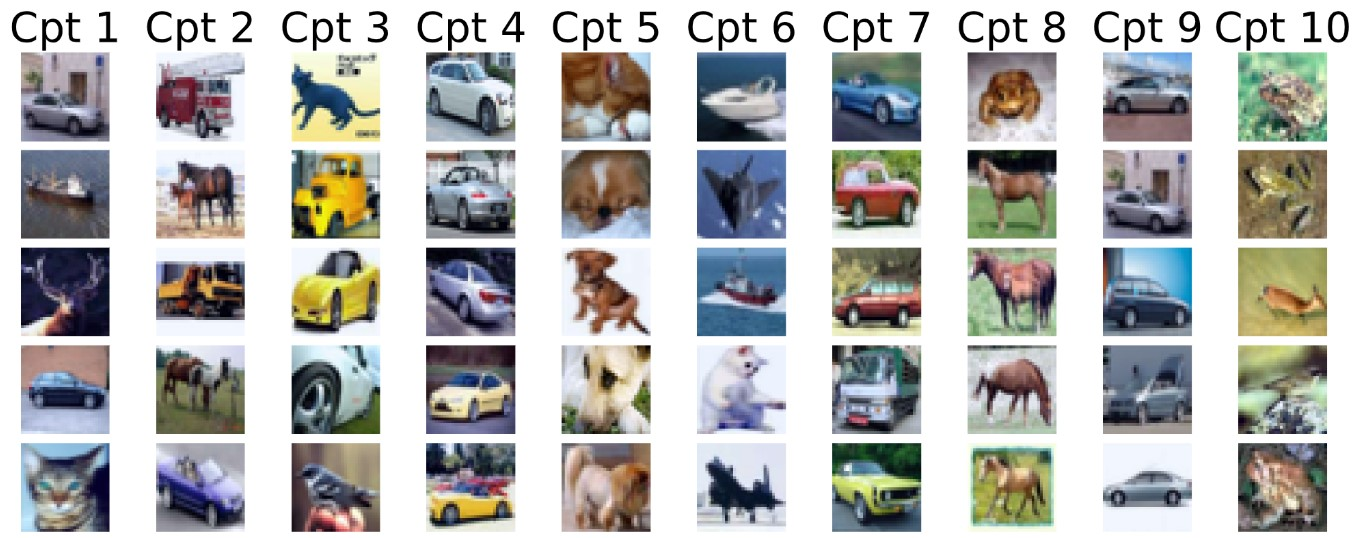
\includegraphics[width=1.0\columnwidth]{images/cgan19.jpg}
    \caption{Top 5 images for CIFAR10 that activate the learnt concepts using cGAN (VGG 19) DAN (B=32, S=5). Eg: Cpt 9 captures a concept corresponding to the grey color, Cpt 10 corresponds to frog skin.}
    \label{fig:cgan19}
\end{figure}

\begin{figure}[h!]
    \centering
    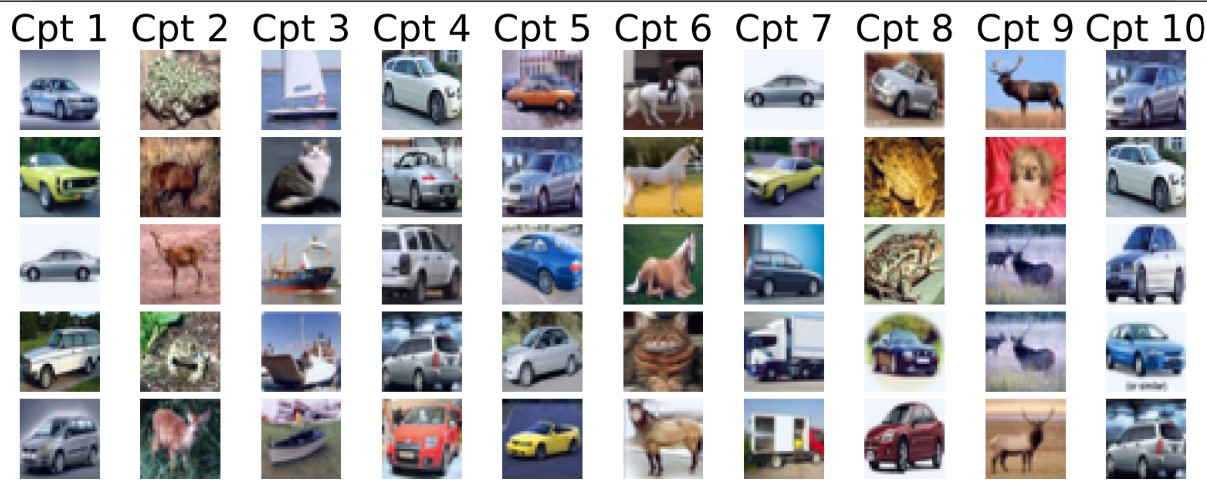
\includegraphics[width=1.0\columnwidth]{images/vcan8.jpg}
    \caption{Top 5 images for CIFAR10 that activate the learnt concepts using Vanilla GAN (VGG 8) ICN  (B=32, S=10). Eg: Cpt 9 corresponds to antlers, Cpt 6 corresponds to shape of legs.}
    \label{fig:vgan8}
\end{figure}

\begin{figure}[h!]
    \centering
    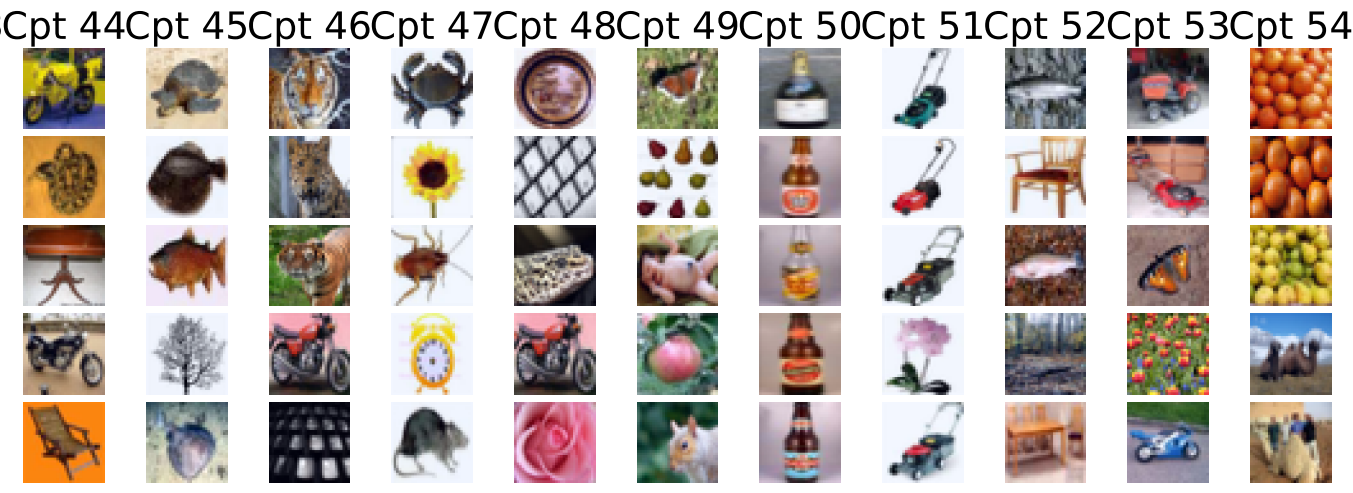
\includegraphics[width=1.0\columnwidth]{images/CGAN_11_1_10_1_cifar100.png}
    \caption{Top 5 images for CIFAR100 that activate the learnt concepts (10 concepts from a subset of 100) using cGAN (VGG 11) PCN  (B=32, S=10). Eg: Cpt 50 corresponds to shape of a bottle, and Cpt 51 corresponds to a lawn-mower.}
    \label{fig:cgan_11_cifar100}
\end{figure}

\begin{figure}[h!]
    \centering
    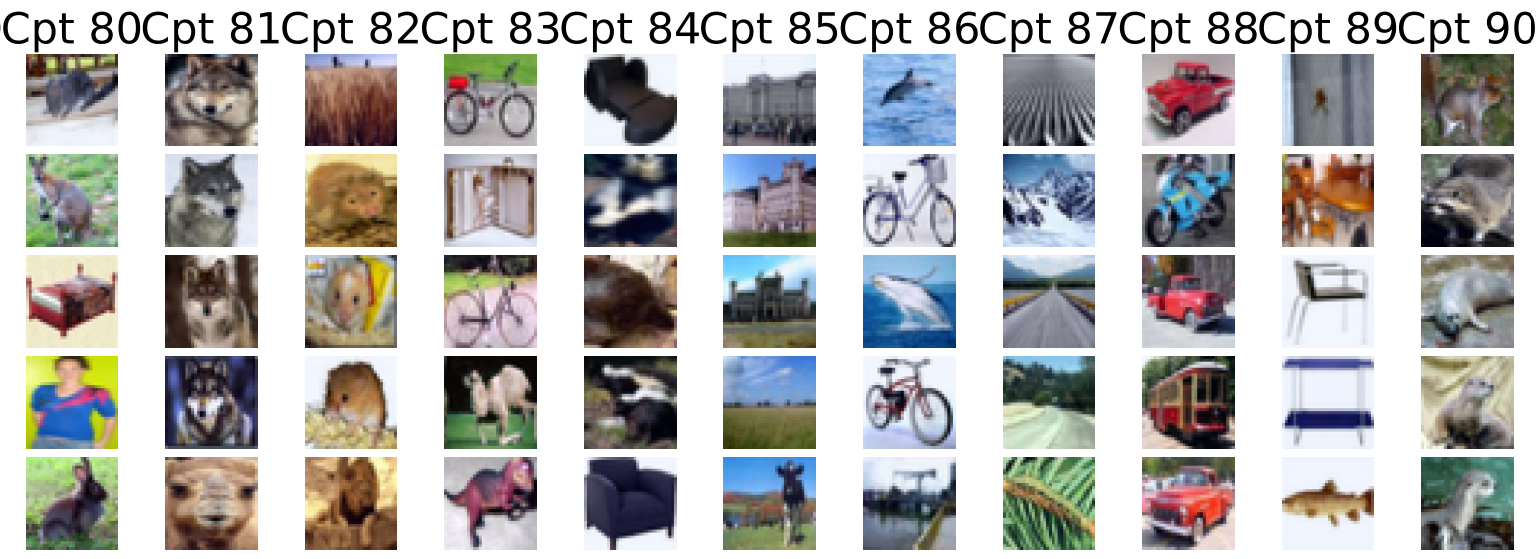
\includegraphics[width=1.0\columnwidth]{images/GAN_11_32_10_1_cifar100.png}
    \caption{Top 5 images for CIFAR100 that activate the learnt concepts (10 concepts from a subset of 100) using Vanilla GAN (VGG 11) DAN (B=32, S=10). Eg: Cpt 81 corresponds to face of a wolf, Cpt 88 corresponds to wheels.}
    \label{fig:cgan_11_cifar100}
\end{figure}

\textbf{cGAN:}\label{sec:cond_gan}
%In the context of cGAN, we will differentiate between different discriminator architectures and choose the best model out each of the architectures with respect to the noise methods.
Here, in addition to a noise size of 10, we also experiment with a noise size of 5 to examine its effect on the framework.
As shown in Table \ref{tab:all_model}, for \textbf{CIFAR10}, using VGG 8, PCN gives the best accuracy of \textbf{91.60\%}. In the case of VGG 11, for a noise size of 10, we get better results using DAN - with an accuracy of \textbf{91.58\%}; whereas for a noise size of 5, we get better results using PCN - with an accuracy of \textbf{91.47\%}. Finally, in the case of VGG 19, DAN gives the best results when using a noise size of 5.
As shown in Table \ref{tab:cifar100_compare}, for \textbf{CIFAR100}, we consistently observe that DAN gives the best results. In the case of VGG 11, using DAN we get the best accuracy of \textbf{65.37\%}. With VGG 19, using DAN we get the best accuracy of \textbf{64.42\%}.

% \subsection{Reviewer Answers}
% For CIFAR100, Our model takes approximately, 0.52 sec for each batch and a total average of 12 minutes for each epoch. In order to compare with our model, \cite{Sarkar2021AFF} took 0.26 sec for each batch and a total average of 6 min for each epoch. \cite{SENN} took 0.84 sec for each batch and a total average of 20 min for each epoch. The model complexity increases significantly with the addition of a GAN and VGG network as discriminator. The improvement is marginal, but the computational time is not significantly larger as compared to \cite{SENN}.

% The main task of our research was to study the how an adversarial nature could be incorporated in an ante-hoc concept learning framework and also study the effects of different noise sampling techniques on the robustness of the framework. Our results seem to be a marginal increase over our baseline, but our empirical study indicates that we can incorporate a generative model into such a framework and receive an improvement in the learning of concepts.

% The noise sampling methods were introduced to study how noise fed into a generator with concepts to generate images that could train the encoder to encode relevant concepts that could be human-interpretable.

% \cite{Sarkar2021AFF} used a simple decoder and L-2 distance loss function to implement and test their theory. We wanted to increase the model complexity to capture richer concepts, as well as improve performance by using a GAN. The adversarial nature of GAN impacts the encoder during the training process. This helps capture more explainable concepts that could be visualized in the figures.
% The discriminator would allow the generated image to represent the original image as close as possible. Moreover, conditioning the GAN over labels additionally helps the network learn better concepts that can be visualized in the figures.

% Increasing the model complexity helps us capture richer concepts that can be validated from the figures. The adversarial nature of GANs impact the encoder during the training process making it capture more explainable concepts.

\end{document}